\iffalse
\let\negmedspace\undefined
\let\negthickspace\undefined
\documentclass[journal,12pt,onecolumn]{IEEEtran}
\usepackage{cite}
\usepackage{amsmath,amssymb,amsfonts,amsthm}
\usepackage{algorithmic}
\usepackage{graphicx}
\usepackage{textcomp}
\usepackage{xcolor}
\usepackage{txfonts}
\usepackage{listings}
\usepackage{enumitem}
\usepackage{mathtools}
\usepackage{gensymb}
\usepackage{comment}
\usepackage{caption}
\usepackage[breaklinks=true]{hyperref}
\usepackage{tkz-euclide} 
\usepackage{listings}
\usepackage{gvv}                                        
\def\inputGnumericTable{}                                 
\usepackage[latin1]{inputenc}                                
\usepackage{color}                                            
\usepackage{array}                                            
\usepackage{longtable}                                       
\usepackage{calc}                                             
\usepackage{multirow}                                         
\usepackage{hhline}                                           
\usepackage{ifthen}                                           
\usepackage{lscape}

\newtheorem{theorem}{Theorem}[section]
\newtheorem{problem}{Problem}
\newtheorem{proposition}{Proposition}[section]
\newtheorem{lemma}{Lemma}[section]
\newtheorem{corollary}[theorem]{Corollary}
\newtheorem{example}{Example}[section]
\newtheorem{definition}[problem]{Definition}
\newcommand{\BEQA}{\begin{eqnarray}}
\newcommand{\EEQA}{\end{eqnarray}}
\newcommand{\define}{\stackrel{\triangle}{=}}
\theoremstyle{remark}
\newtheorem{rem}{Remark}
\begin{document}

\bibliographystyle{IEEEtran}
\vspace{3cm}

\title{GATE IN 43}
\author{EE23BTECH11022 - G DILIP REDDY}
\maketitle

\bigskip

\renewcommand{\thefigure}{\arabic{figure}}
\renewcommand{\thetable}{\arabic{table}}
\textbf{Question}:\\
The magnitude and phase plots shown in the figure match with the transfer-
function
\begin{figure}[h]
    \centering
    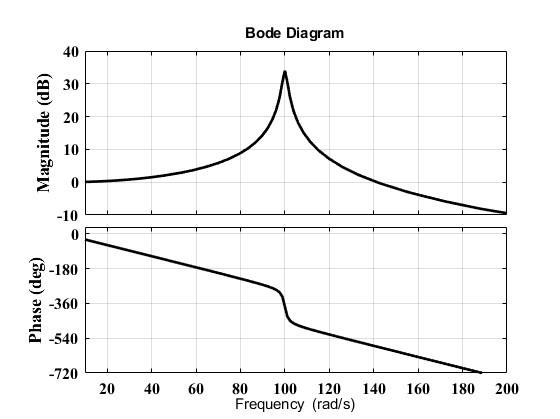
\includegraphics[width=\columnwidth]{2023/IN/43/figs/question.png}
\end{figure}\\
\renewcommand{\labelenumi}{\alph{enumi})}
\begin{enumerate}
\item $\frac{10000}{s^2+2s+10000}$\\
\item $\frac{10000}{s^2+2s+10000}e^{-0.05s}$\\
\item $\frac{10000}{s^2+2s+10000}e^{-0.5\times10^{-12}s}$\\
\item $\frac{100}{s^2+2s+100}$
\end{enumerate}
\hfill{(GATE IN 2023)}
\\\\
\solution
\fi
Drawing bode plots for four options.\\
\begin{align}
\implies H\brak{s}=\frac{k}{s ^{2}+2s+k}e^{as}\\
H\brak{j\omega}=\frac{k}{k-\omega ^2+2j\omega}e^{aj\omega}\\
\abs{H\brak{j\omega}}=\frac{k}{\sqrt{\brak{k-\omega ^2}^2+4\omega^2}}\\
\implies \phi\brak{H\brak{j\omega}}=\brak{-\tan^{-1}{\brak{\frac{2\omega}{k-\omega^2}}-a\omega}}
\end{align}
From the graphs , the answer is b

\begin{figure}[h]
    \centering
    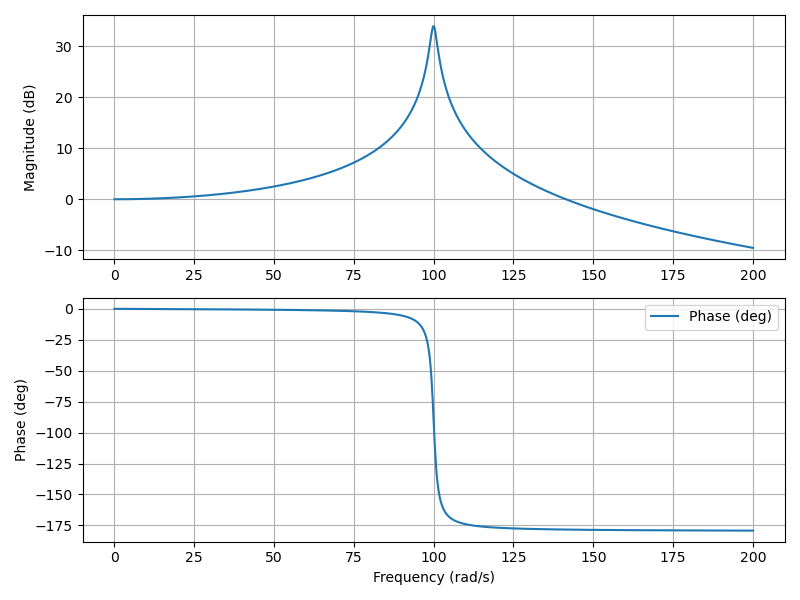
\includegraphics[width=\linewidth]{2023/IN/43/figs/A.png}
    \caption{Bode plot of a $\frac{10000}{s^2+2s+10000}$}
\end{figure}
\begin{figure}[h]
    \centering
    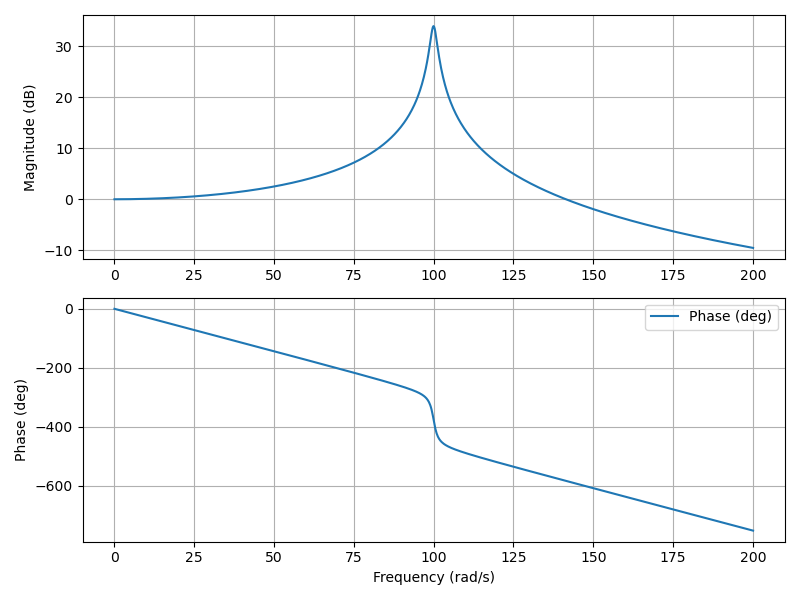
\includegraphics[width=\linewidth]{2023/IN/43/figs/B.png}
    \caption{Bode plot of a $\frac{10000e^{-0.05s}}{s^2+2s+10000}$}
\end{figure}
\begin{figure}[h]
    \centering
    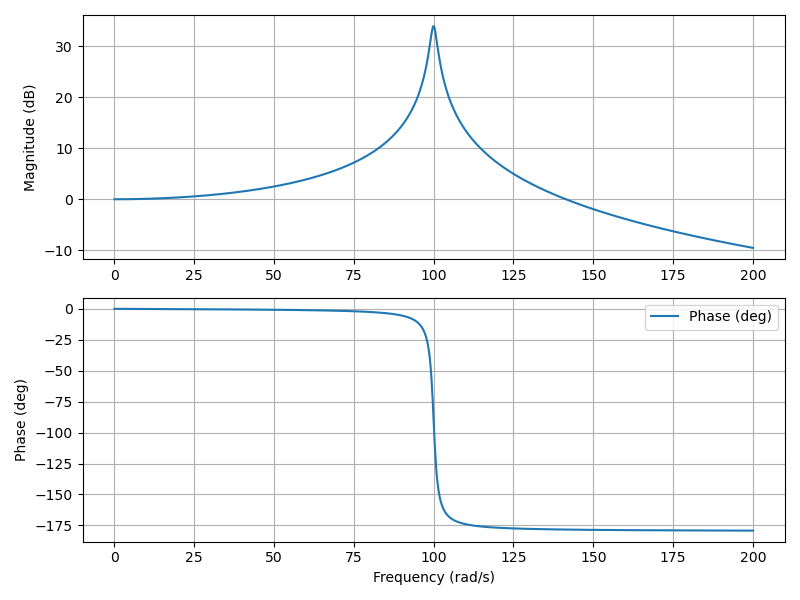
\includegraphics[width=\linewidth]{2023/IN/43/figs/C.png}
    \caption{Bode plot of a $\frac{10000e^{0.5\times10^{-12}s}}{s^2+2s+10000}$}
\end{figure}
\begin{figure}[h]
    \centering
    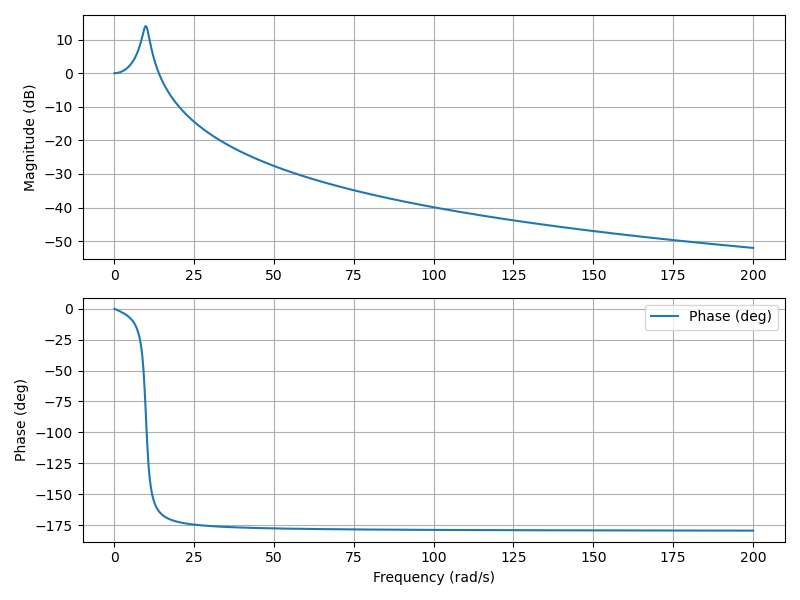
\includegraphics[width=\linewidth]{2023/IN/43/figs/D.png}
    \caption{Bode plot of a $\frac{100}{s^2+2s+100}$}
\end{figure}
%\end{document}
